\documentclass[conference]{IEEEtran}

\IEEEoverridecommandlockouts                              % This command is only needed if 
                                                          % you want to use the \thanks command

\overrideIEEEmargins                                      % Needed to meet printer requirements.

% See the \addtolength command later in the file to balance the column lengths
% on the last page of the document

\usepackage{amssymb}
\setcounter{tocdepth}{3}
\usepackage{graphicx}
\usepackage[fleqn]{amsmath}
\usepackage{url}
\usepackage{amsmath} % assumes amsmath package installed
\usepackage{amssymb}  % assumes amsmath package installed
\usepackage{algorithm}			% pacchetti per i pezzi di pseudocodice
\usepackage{algorithmic}		% pacchetti per i pezzi di pseudocodice

\usepackage{float}		% pacchetto per figure e tabelle

% Lettere accentate:
\usepackage[utf8x]{inputenc}


%\usepackage{mathptmx} % assumes new font selection scheme installed
%\usepackage{times} % assumes new font selection scheme installed


% correct bad hyphenation here
\hyphenation{op-tical net-works semi-conduc-tor}


\begin{document}
%
% paper title
% can use linebreaks \\ within to get better formatting as desired
\title{SPQR@Work: Team Description Paper}

\author{\IEEEauthorblockN{Marco Imperoli, Harold Agudelo, Daniele Evangelista, Ahmad Rjoub,\\Valerio Sanelli, Alberto Pretto and Daniele Nardi}\\
\IEEEauthorblockA{Department of Computer, Control, and Management Engineering\\``Antonio Ruberti``, Sapienza University of Rome, Italy.\\ Email: {\tt\small marcoimperoli@gmail.com, agudeloramirez.1644608@studenti.uniroma1.it,}\\ 
{\tt\small evangelista.1665872@studenti.uniroma1.it, ahmad000rjoub@yahoo.com,}\\
{\tt\small valerio.sanelli@gmail.com, \{pretto,nardi\}@dis.uniroma1.it}\\
Website: {\tt\small http://www.dis.uniroma1.it/~labrococo/SPQRWork}}}

% make the title area
\maketitle

\begin{abstract}
%\boldmath
The SPQR@Work team is a spin-off of the S.P.Q.R. RoboCup team of the Department of Computer, Control, and Management Engineering “Antonio Ruberti” at Sapienza University of Rome, created to participate at the RoCKIn@Work competition.\\
This document describes the scientific background, the team members' competences and the employed robot hardware and software that the SPQR@Work team will exploit if it will be accepted to participate to the 2015 RoCKIn competition event.
\end{abstract}

\section{Introduction}
% no \IEEEPARstart
The SPQR@Work team has been founded as an offshoot of the S.P.Q.R. RoboCup team, that is involved in RoboCup competitions since 1998 in different leagues :
\begin{itemize}
\item Middle-size 1998-2002;
\item Four-legged 2000-2007;
\item Real-Rescue robots since 2003;
\item Virtual-Rescue robots since 2006;
\item Standard Platform League since 2008
 \end{itemize}

The team involves both PhD students and graduated students, members of the Cognitive Cooperating Robots laboratory, supervised by Dr. Alberto Pretto and Prof. Daniele Nardi.\\ 

SPQR@Work goals are the following:
\begin{itemize}
 \item Set up a team to successfully compete in RoCKIn@Work competition.
 \item Propose and test new techniques for (1) RGB-D object recognition and localization (2) Object manipulation and grasping (3) Robot Navigation and Planning.
 \item Promote teaching initiatives to foster the participation of students in research on intelligent mobile robotics.
\end{itemize}
 
\section{Team Presentation}
\subsection{Team Details}

\begin{itemize}
 \item \textbf{Team name:} SPQR@Work
 \item \textbf{Selected track:} RoCKIn@Work
 \item \textbf{Team members:} Harold Agudelo, Daniele Evangelista, Ahmad Rjoub, Valerio Sanelli
  \item \textbf{Team leader:} Marco Imperoli
 \item \textbf{Advisors:} Alberto Pretto, Daniele Nardi
 \item \textbf{Robot:} 1 Kuka youBot
\end{itemize}

\subsection{Involved Institutions}
\begin{figure}[t!]
\begin{center}
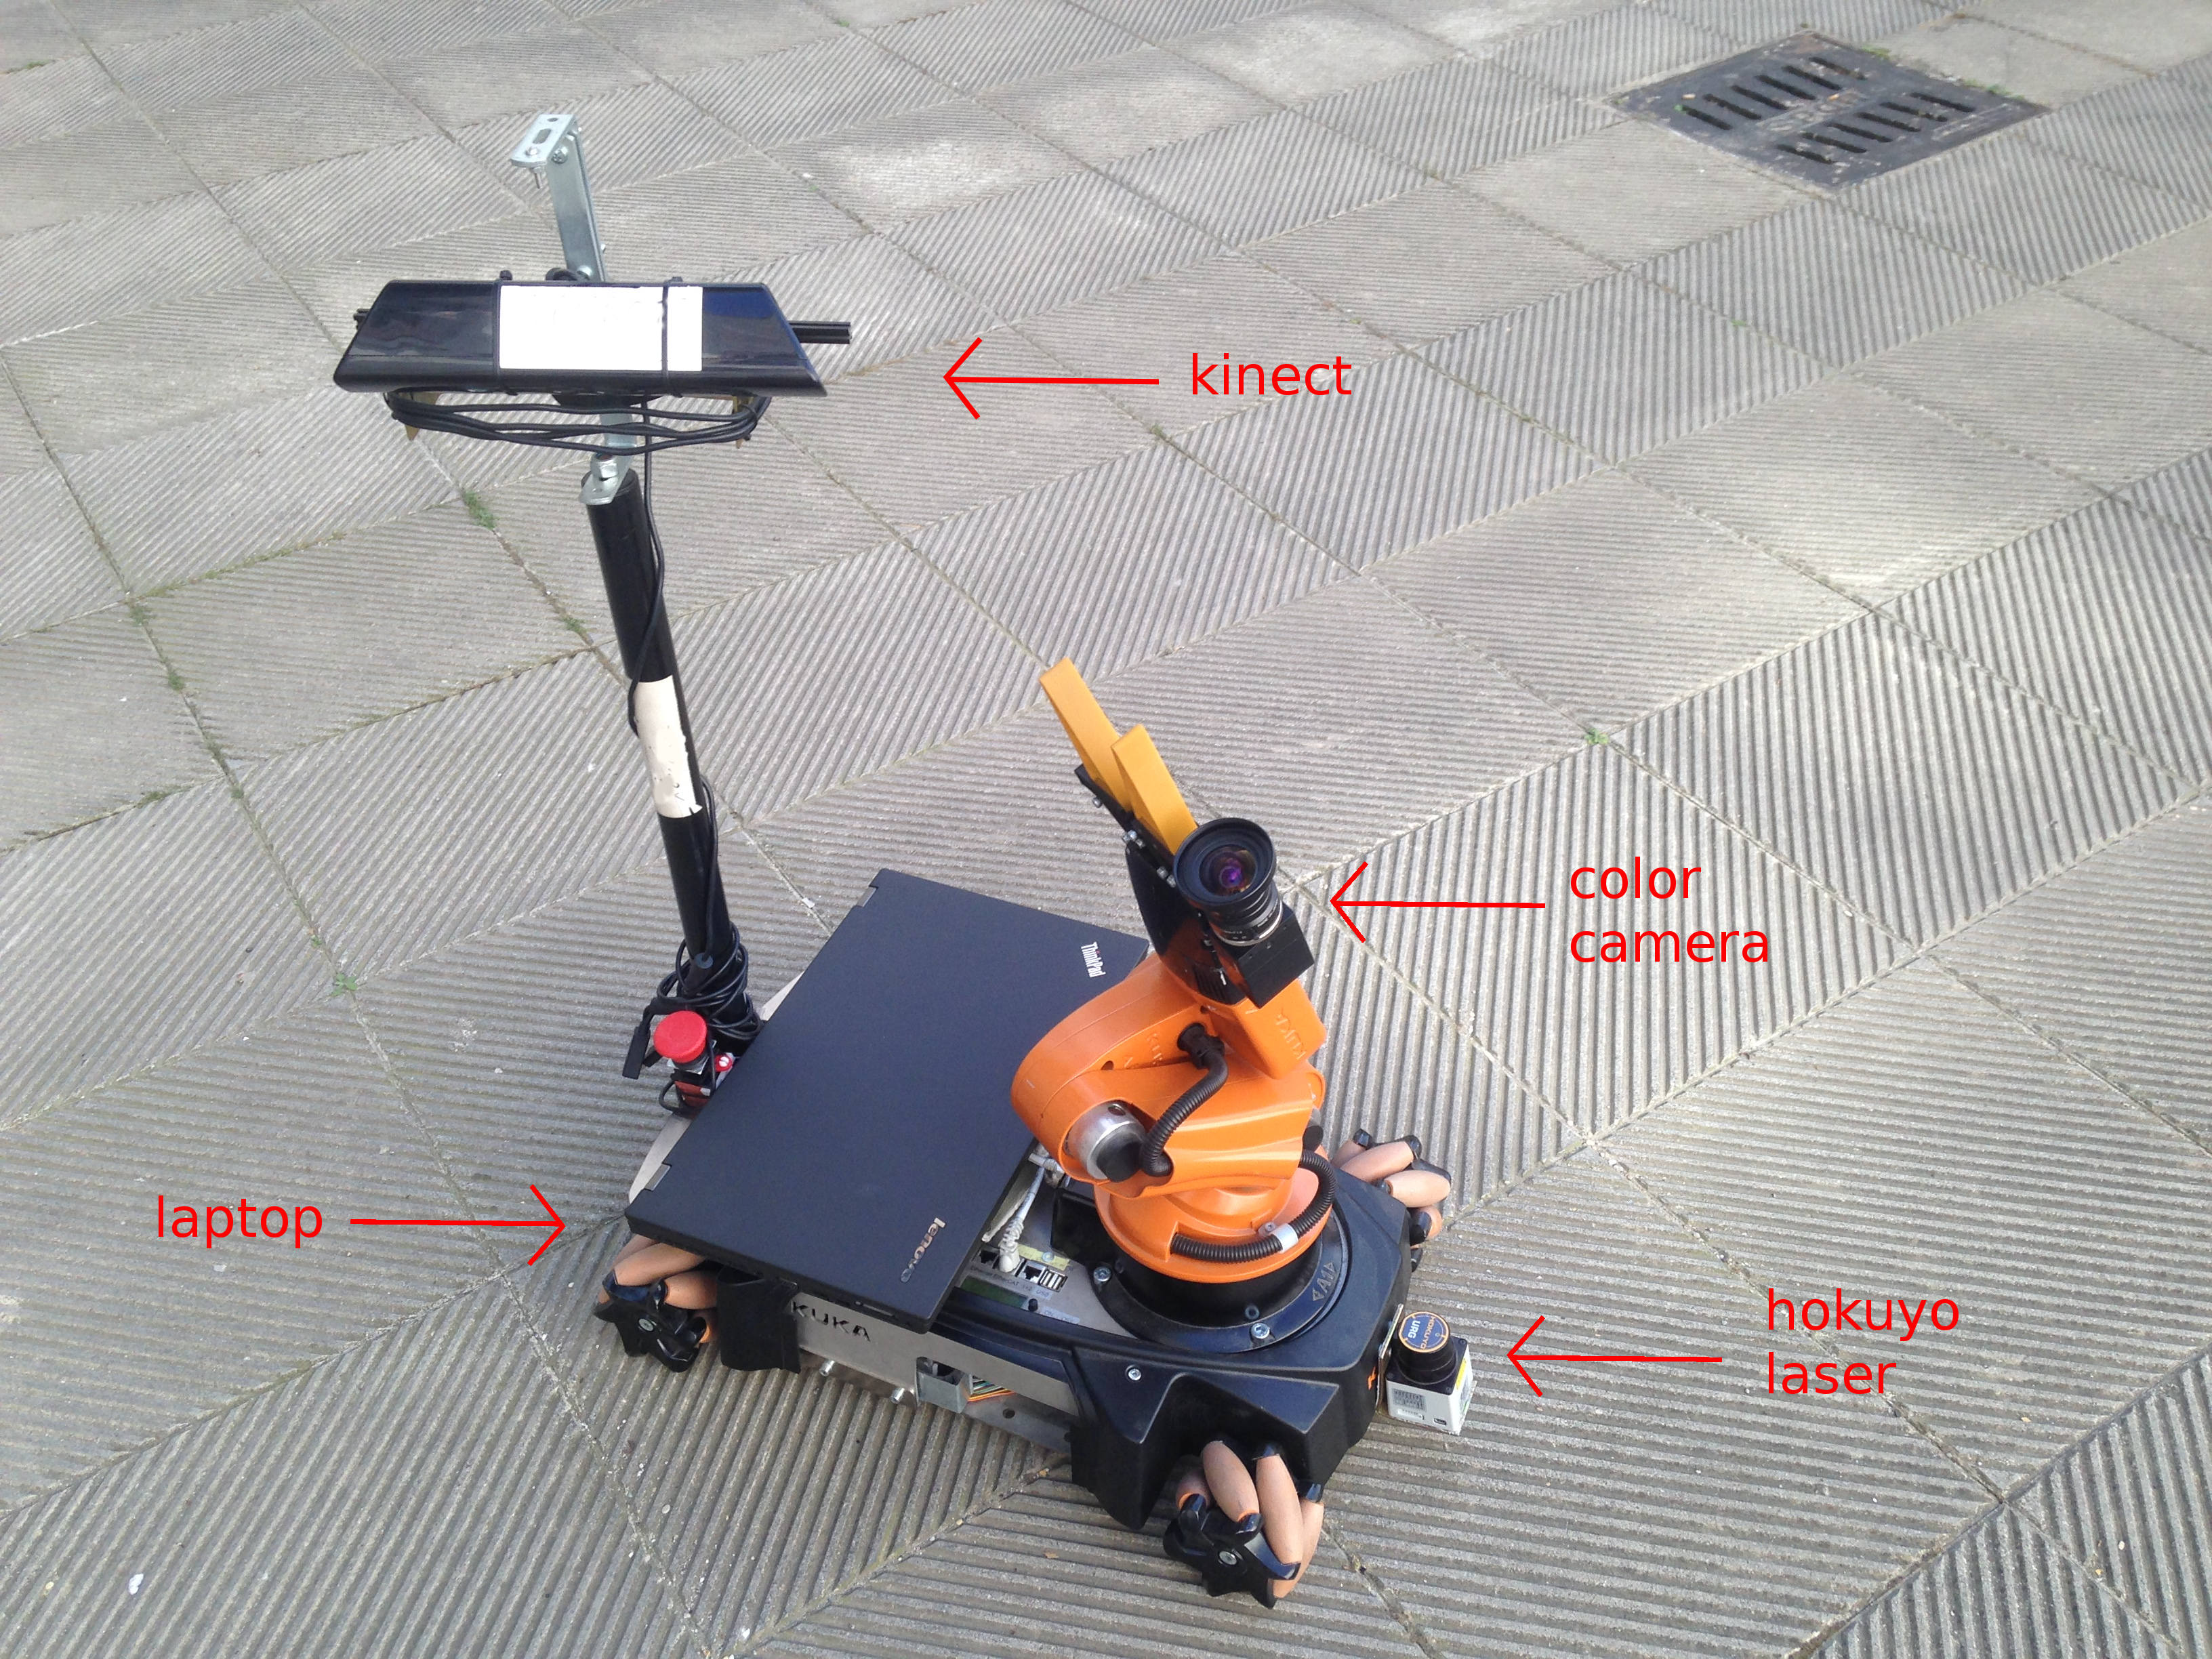
\includegraphics[width=\linewidth]{images/kuka.JPG}
\end{center}
\caption{The SPQR@Work robot: the laptop is used for computationally expensive tasks (localization, mapping, object recognition, \dots) while the internal standard Intel Atom PC is used for low-level motions controls (platform and arm).}\label{fig:robot}
\end{figure}

\subsubsection{RoCoCo} The laboratory RoCoCo (Cognitive Cooperating Robots) is located at DIAG (Dipartimento di Ingegneria Informatica, Automatica e Gestionale) of Sapienza University of Rome, Italy.
The research developed at RoCoCo laboratory is in the area of Artificial Intelligence and Robotics: Lab RoCoCo has a strong background in knowledge representation and reasoning, cognitive robotics, information fusion, mapping and localization, object recognition and tracking. multi-robot coordination, robot learning, stereo-vision, vision-based people detection. RoCoCo has been involved in RoboCup competitions since 1998 in different leagues.\\

\subsection{Competence of Team Members}

\subsubsection*{Marco Imperoli}

Imperoli is a first year Ph.D. student at Sapienza University of Rome. 
In 2015 he received the Master degree in Artificial Intelligence and Robotics Engineering. 
His research is mainly focused on active perception problems for object recognition and accurate full 3D objects pose estimation.  

\subsubsection*{Harold Agudelo}

Agudelo is a second year student of the Master degree in Artificial Intelligence and Robotics Engineering at Sapienza University of Rome. In 2013 he received the Electronic Engineer degree from Universidad del Norte, Colombia. His areas of interest are related with Artificial Intelligence in domotics. 

\subsubsection*{Daniele Evangelista}
% This is only a Draft - needs to be updated - D.E.
Evangelista is currently attending the second year of the Master degree in Articial Intelligence and Robotics at Sapienza University, in Rome. In October 2014 he got the bachelor degree in Informatics and Telecommunications engineering at University of Cassino. He is also the co-founder and CEO of \emph{alibabyte software house S.r.l.s.}, an italian company mainly focused on web, desktop and mobile software development. His main interests are in Machine Learning and Artificial Intelligence in robotics applications.

\subsubsection*{Ahmad Rjoub}

Ahmad Irjoob joined Sapienza university in Sep 2014  Artificial intelligence and robotics after he get his bachelor degree in Telecommunication engineer from Yarmook university in Jordan ,and Irjoob so interest in network field and he always think to apply this in robotic.

\subsubsection*{Valerio Sanelli}

Valerio Sanelli is a Master student of Artificial Intelligence and Robotics at la Sapienza, University of Rome.
He received the Bachelor Degree in Computer Engineering at la Sapienza in 2013.
He is mainly focused on Artificial Intelligence, with particular  emphasis on Robot Learning, Automated Reasoning and Vision systems.

\subsubsection*{Alberto Pretto}

Pretto is Assistant Professor at Sapienza University of Rome since October 2013. 
He received his Ph.D. degree in October 2009 from the University of Padua, where he worked as a postdoctoral researcher at the Intelligent Autonomous Systems Lab (Department of Information Engineering). 
In 2005, he was one of the funders of IT+Robotics Srl, a spin-off company of the University of Padua working on robotics and machine vision. 
Alberto Pretto's main research activities include vision-based 3D reconstruction, visual-inertial navigation, and object recognition.

\subsubsection*{Daniele Nardi}

Nardi is Full Professor at DIS, where he was employed since 1986. His current research interests are in the field of artificial intelligence and cognitive robotics. He is Trustee of RoboCup and currently the president of the RobotCup Federation.  From 2005-2008, he also served as the co-chair of IEEE Technical Committee of International Workshop on Safety, Security and Rescue Robotics.  He is active in the context of autonomous rescue robots and successfully coordinated a team participating on several editions of RoboCup Rescue since the year 2002.  
Nardi received the ``IJCAI-91 Publisher's Prize'' and the prize ``Intelligenza Artificiale 1993'' from the Associazione Italiana per l'Intelligenza Artificiale (AI*IA).

\subsection{RoCKIn Events participations}

Imperoli participated at the RoCKIn Camp 2014, RoCKIn Competition 2015, and RoCKIn Camp 2015, with the ``SPQR Team''. In RoCKIn Camp 2014, ``SPQR'' won in ex-aequo with another team the ``Best Practical in Perception'' award.

\section{Robot Description}

\subsection{Hardware Configuration}

The SPQR@Work robot (Fig.~\ref{fig:robot}) is a KUKA youBot with the following sensor suite:

\begin{itemize}
 \item A frontal Hokuyo laser scanner, to be used for navigation and obstacles avoidance tasks
 \item A Kinect RGB-D sensor: the area viewed by the kinect includes the working area of the arm, in order to perform object manipulation tasks without robot motions
 \item An on-board laptop (other than the internal standard Intel Atom PC) running Linux Ubuntu 14.04, to be used to execute the perception and planning tasks (e.g., navigation and object recognition)
 \item A color USB3 high-resolution camera on the 5th joint of the manipulator for accurate object localization
\end{itemize}
 
\subsection{Software Configuration}

The SPQR@Work software infrastructure is based on the ROS Indigo middleware running on Ubuntu 14.04, nevertheless most of the developed software tools are stand-alone, middleware-agnostic: packages are integrated within ROS by means of suitable wrappers.\\
The navigation stack is based on particle filter based localization and mapping algorithms, provided by the ROS AMCL and GMapping packages, the latter implemented by one member of the laboratory RoCoCo.  Tha base motion planning task is accomplished using two different subsystems (see Fig.~\ref{fig:intro_navigation}):
\begin{itemize}
 \item A global planner, which provides the global path to follow, based on the standard MoveBase ROS package;
 \item A custom-built local planner, which, given the global plan and a costmap, produces
velocity commands to send to the mobile base controller.
\end{itemize}
Our ad hoc local planner is based on artificial potential fields, designed for holonomic mobile robots.

\begin{figure}[h!]
\begin{center}
\begin{minipage}[b]{0.6\linewidth}
	\begin{center}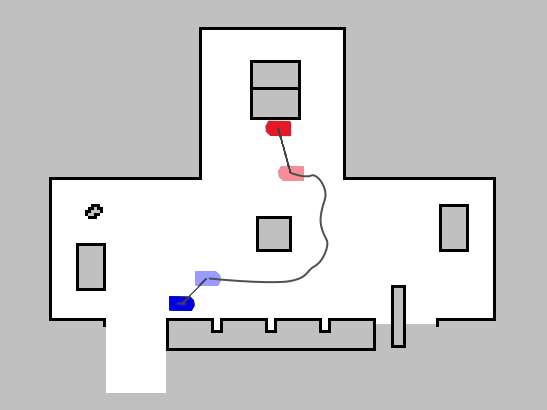
\includegraphics[angle=0,width=\linewidth]{images/navigation.png}\end{center}
\end{minipage}\hfill
\end{center}
\caption{An example of navigation path (dark gray). The curved portion of the entire path is computed by the primary navigation planner. Our potential fields based planner is used for approaching the final target (red) and for sliding away from obstacles at the beginning of the navigation task (blue).}\label{fig:intro_navigation}
\end{figure}

We use a custom-built module also for the manipulation and the grasping tasks: the arm motion planner we propose is able to plan accurate trajectories assuming that the best way to grasp an object disposed in an crowded environment is to let the gripper follows a straight line in the Cartesian space towards the object of interest.\\

Object recognition and localization is obtained using reliable algorithms that exploit both vision features and depth information (Sec.~\ref{sec:object_rec}). This module includes a pipeline of processing blocks (Fig.~\ref{fig:pipeline}): the pipeline includes processing blocks for sub-sampling, clustering, noise reduction, and 2D and 3D features detection and descriptors. The model matching step is performed associating the extracted features with features pre-computed from a rigid template (e.g., the CAD model) of the object. The result is a set of object candidates, that is refined using an novel object registration strategy. \\

The decision making stack is based on a finite state machine implemented with the ROS Actionlib,

\begin{figure*}[t!]
\begin{center}
\includegraphics[angle=0,width=\linewidth]{images/pipeline.png}
\end{center}
\caption{The SPQR@Work object recognition and localization pipeline.}\label{fig:pipeline}
\end{figure*}


Currently, the SPQR@Work robot is able to:

\begin{itemize}
 \item Localize itself and safely navigate toward a selected target area
 \item Detect QR code-like markers using vision
 \item Recognize and localize objects using RGB-D sensors, using the techniques proposed in \cite{antonelloVISIGRAPP2014} and \cite{prettoCASE2013}
 \item Perform simple visual servoing and manipulation tasks (e.g., pick and place task, ``cutting a string'' task, \dots)
\end{itemize}

 
\section{Research areas and Contributions}\label{sec:research}

Several research areas are involved in the SPQR@Work team development, and some novel contributions have been proposed. Among others, PWN (Sec.~\ref{sec:pwn}), a semantic mapping and learning system (Sec.~\ref{sec:semantic_map}) and a flexible 3D localization system for industrial bin-picking (Sec.~\ref{sec:object_rec}).


\subsubsection{Object Recognition and Localization}\label{sec:object_rec}
A reliable and accurate object recognition system is an essential prerequisite to successfully compete in the RoCKIn competitions. The SPQR@Work team members presented a robust and flexible vision system for 3D localization of objects for industrial robots \cite{prettoCASE2013} (Fig.~\ref{fig:obj_rec}). This system can estimate the 6 degrees of freedom (DoF) pose of planar objects from a single 2D image.
The localization software is based on a two step strategy: i) a candidate selection step based on a well-engineered voting scheme ii) a refinement and best match selection step based on a robust iterative optimize-and-score procedure. During this second step, a novel strategy called search-in-the-stack is employed, that avoids the optimization from being stuck on local minima (representing false positives) created when objects are almost regularly stacked.

\subsubsection{Obstacle Avoidance and Manipulation}\label{sec:manipulation}
In order to obtain a reliable robot navigation, SPQR@Work team members implemented an efficient obstacle avoidance system for mobile robots equipped with range finder sensors, based on the online computation of local artificial potential fields. \newline In the field of manipulation, an effective framework for handling task priority of redundant manipulators has been studied and developed.
\begin{figure}[t!]
\begin{center}
\includegraphics[angle=0,width=\linewidth]{images/result_number01_small.jpg}
\end{center}
\caption{Final results of the proposed localization system.}\label{fig:obj_rec}
\end{figure}

\section{Reusability and Relevance to Industrial Robotics}

\begin{itemize}
 \item PWN (Sec.~\ref{sec:pwn}) became a basic block for a novel traversability analysis algorithm described by Bogoslavskyi et al. in~\cite{bogoslavskyi-ECMR-13}.
 \item The proposed object recognition and localization systems (Sec.~\ref{sec:object_rec}) is currently installed in seven real world industrial plants \footnote{E.g., https://www.youtube.com/watch?v=jqhuEjnDdfI}, with different setups, working with hundreds of different models and successfully guiding the manipulators to pick several hundreds of thousands of pieces per year. 
 \item The proposed task priority manager (Sec.~\ref{sec:manipulation}) is currently implemented inside a real 3D industrial simulator for the off-line programming of workcells and machines with several axis.  \footnote{http://www.it-robotics.it/products/3d-simulation/workcellsimulator/?lang=en}
\end{itemize}

\bibliographystyle{IEEEtran}
\bibliography{bibliography} 

% that's all folks
\end{document}